\subsubsection{Minuta de reunião (02-Setembro-2015)}

\begin{tabbing}
  Local \= xxx \kill
  Local \> : LEAD \\
  Data  \> : 02 de Setembro de 2015 \\
  Hora  \> : 13:00
\end{tabbing}

%---------------------------------------------------------------------
\participantes{
  \alana
  \gabriel,
  \julia,
  \estevão,
  \elael,
  \renan,
  \ramon.

}

\textbf{Aprovação da minuta}

\textbf{Update semanal do Projeto EMMA}
   							
\textbf{\alana.} 
	\begin{itemize}
		\item \textbf{Tarefas concluídas:}
			\begin{itemize}    
				\item Viagem Jirau.
				\item Relatório Auditoria.
			\end{itemize}
		
		\item \textbf{Novas tarefas:}
			\begin{itemize} 
				\item Ofício Viagem Jirau: passagens, diárias e locação de carros.
				\item Cronograma de viagem.
				\item Justificativa Ramon.
			\end{itemize}
	\end{itemize}   		
						
\textbf{\gabriel.} 
	\begin{itemize}
			\item Incluiu novas cotações para sensores Leica
			\item Implementou driver ROS para ROCK no Laser Scan.
			\end{itemize}
		
		\item \textbf{Novas tarefas:}
			\begin{itemize} 
				\item Continuar Point Cloud Alignment.
				\item Apresentação sobre alinhamento de pás e braço mecânico.
			\end{itemize}

					
			
   \textbf{\estevão.} 
	\begin{itemize}
		\item \textbf{Tarefas concluídas:}
			\begin{itemize}  
			  \item Contratou serviço para maquete, prazo de entrega de um mês.
			  \item Apresentação de Base de com trilho e suporte.
			\end{itemize}
		
		\item \textbf{Novas tarefas:}
			\begin{itemize} 
				\item Estado da arte de soluções modulares para bases robóticas em ambientes de difícil acesso.
			\end{itemize}
	\end{itemize}

	  \textbf{\renan.} 
	\begin{itemize}
		\item \textbf{Tarefas concluídas:}
			\begin{itemize}    
				\item Apresentou a aplicação de hardcoating Frame by Frame no OpenRave. 
				\item Estudo aproximando e afastando o robô da pá, na base criada por
				Estevão.
				\item Apresentou o início da pesquisa Dinâmica,
			\end{itemize}
		
		\item \textbf{Novas tarefas:}
			\begin{itemize} 
			    \item Continuar com estudo de Dinâmica
			\end{itemize}
	\end{itemize}	
	
	
	  \textbf{\elael.} 
	\begin{itemize}
		\item \textbf{Tarefas concluídas:}
			\begin{itemize}    
				\item Cotações para Point Laser. 
			\end{itemize}
		
		\item \textbf{Novas tarefas:}
			\begin{itemize} 
			    \item Continuar estudo de alinhamento de Point Cloud.
			\end{itemize}
	\end{itemize}			
			
			
   \textbf{\julia.} 
	\begin{itemize}
		\item \textbf{Tarefas concluídas:}
			\begin{itemize}    
				\item Apresentação processo de trablho para EMMA Fase 1: Descoberta para o
				time.
			\end{itemize}
		
		\item \textbf{Novas tarefas:}
			\begin{itemize} 

			    \item Apresentar Fase 2: Design.
			\end{itemize}
	\end{itemize}		



\textbf{Agenda para a próxima reunião:}
  \begin{itemize}
    \item Resultado de pesquisas individuais.
    \item Novas tarefas \& recomendações.
  \end{itemize}


\vspace{5mm}%
\parbox[t]{70mm}{
  Aprovado por: \\[5mm]
  \centering
  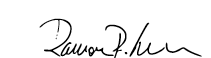
\includegraphics[width=65mm]{figs/logo/assinatura-ramon.png} \\[-4mm]
  \rule[2mm]{70mm}{0.1mm} \\
  \ramon \\[1mm]
  Coordenador do Projeto \\
}

%---------------------------------------------------------------------
\fim